\documentclass[12pt,a4paper]{article}

% ------------------------------------------------------------
% Encoding, language, fonts
% ------------------------------------------------------------
\usepackage[T1]{fontenc}
\usepackage[utf8]{inputenc}
\usepackage[ngerman,english]{babel}
\usepackage{lmodern}
\usepackage{microtype}

% ------------------------------------------------------------
% Page layout
% ------------------------------------------------------------
\usepackage{pdflscape}

% ------------------------------------------------------------
% Mathematics, tables, figures
% ------------------------------------------------------------
\usepackage{amsmath,amssymb,amsfonts,amsthm}
\usepackage{mathtools}
\usepackage{array,booktabs}
\usepackage{float}
\usepackage{flafter}
\usepackage{graphicx}
\usepackage{caption}
\usepackage{subcaption}
\usepackage{siunitx}
\graphicspath{{figures/}}

% ------------------------------------------------------------
% Diagrams and colours
% ------------------------------------------------------------
\usepackage[dvipsnames]{xcolor}
\usepackage{tikz}
\usetikzlibrary{arrows.meta,positioning,fit,calc}
\usepackage{enumitem}

% ------------------------------------------------------------
% Plots
% ------------------------------------------------------------
\usepackage{pgfplots}
\pgfplotsset{compat=1.17}

% ------------------------------------------------------------
% Bibliography
% Compile with: pdfLaTeX -> Biber -> pdfLaTeX -> pdfLaTeX
% ------------------------------------------------------------
\usepackage{csquotes}
\usepackage[backend=biber,style=numeric,sorting=none]{biblatex}
\addbibresource{references.bib}

% ------------------------------------------------------------
% Code listings
% ------------------------------------------------------------
\usepackage{upquote}
\usepackage{listings}

\definecolor{codebackground}{RGB}{248,248,248}
\definecolor{codegray}{gray}{0.45}

\lstdefinestyle{commoncodestyle}{
    inputencoding=utf8,
    extendedchars=true,
    backgroundcolor=\color{codebackground},
    basicstyle=\ttfamily\footnotesize,
    keywordstyle=\bfseries\color{blue!60!black},
    commentstyle=\itshape\color{green!40!black},
    stringstyle=\color{red!55!black},
    numbers=left,
    numberstyle=\tiny\color{codegray},
    stepnumber=1,
    numbersep=5pt,
    frame=single,
    framerule=0.3pt,
    framesep=3pt,
    rulecolor=\color{black!30},
    breaklines=true,
    breakatwhitespace=false,
    breakindent=1em,
    breakautoindent=true,
    postbreak=\mbox{\textcolor{codegray}{$\hookrightarrow$}\space},
    showstringspaces=false,
    columns=flexible,
    keepspaces=true,
    tabsize=4,
    captionpos=t,
    upquote=true,
    linewidth=\linewidth,
    xleftmargin=0pt,
    xrightmargin=0pt,
    literate={é}{{\'e}}1 {É}{{\'E}}1 {ä}{{\"a}}1 {ö}{{\"o}}1 {ü}{{\"u}}1 {Ä}{{\"A}}1 {Ö}{{\"O}}1 {Ü}{{\"U}}1 {ß}{{\ss}}1 {–}{{--}}1 {—}{{---}}1 {’}{{'}}1 {‘}{{'}}1 {“}{{``}}1 {”}{{''}}1 {≤}{{$\leq$}}1 {≥}{{$\geq$}}1 {→}{{$\to$}}1
}

\lstdefinestyle{pythonstyle}{
    style=commoncodestyle,
    language=Python
}

\lstdefinestyle{bashstyle}{
    style=commoncodestyle,
    language=bash
}

\lstdefinestyle{pythontextstyle}{
    style=pythonstyle,
    basicstyle=\ttfamily\footnotesize,
    numbers=none,
    frame=single,
    framerule=0.3pt,
    breaklines=true,
    breakatwhitespace=false,
    captionpos=t
}

\lstset{style=pythontextstyle}

\renewcommand{\lstlistingname}{Code Listing}
\renewcommand{\lstlistlistingname}{List of Code Listings}

% ------------------------------------------------------------
% Hyperlinks and cross-references
% ------------------------------------------------------------
\usepackage{xurl}
\usepackage[hidelinks]{hyperref}
\usepackage[capitalise,noabbrev]{cleveref}

% ------------------------------------------------------------
% Theorems and notation used in the paper
% ------------------------------------------------------------
\theoremstyle{plain}
\newtheorem{proposition}{Proposition}
\theoremstyle{definition}
\newtheorem{definition}{Definition}

\newcommand{\code}[1]{\texttt{#1}}
\newcommand{\FD}{FD}
\newcommand{\FDS}{FD-S}

% Generated benchmark values used throughout the paper
% Generated by benchmark/run.py -- do not edit by hand.
\newcommand{\NScen}{10}
\newcommand{\NFramesScen}{90}
\newcommand{\NFramesCtrl}{900}
\newcommand{\NSeeds}{10}
\newcommand{\RefreshK}{15}
\newcommand{\NTransitions}{8900}
\newcommand{\YoloMs}{698}
\newcommand{\GateRecallFD}{0.996}
\newcommand{\GateFprFD}{0.206}
\newcommand{\GatePrecFD}{0.832}
\newcommand{\GateRecallCIFD}{[0.993, 0.997]}
\newcommand{\GateFprCIFD}{[0.195, 0.219]}
\newcommand{\GateMsFD}{1.43}
\newcommand{\CostRatioFD}{0.0020}
\newcommand{\BreakEvenFD}{0.998}
\newcommand{\GateFprJitterFD}{0.996}
\newcommand{\GateFprIllumFD}{0.022}
\newcommand{\GateRecallSmallFD}{1.000}
\newcommand{\GateRecallJitterWalkFD}{1.000}
\newcommand{\GateRecallFDS}{0.996}
\newcommand{\GateFprFDS}{0.014}
\newcommand{\GatePrecFDS}{0.987}
\newcommand{\GateRecallCIFDS}{[0.993, 0.997]}
\newcommand{\GateFprCIFDS}{[0.011, 0.018]}
\newcommand{\GateMsFDS}{7.25}
\newcommand{\CostRatioFDS}{0.0104}
\newcommand{\BreakEvenFDS}{0.990}
\newcommand{\GateFprJitterFDS}{0.069}
\newcommand{\GateFprIllumFDS}{0.000}
\newcommand{\GateRecallSmallFDS}{1.000}
\newcommand{\GateRecallJitterWalkFDS}{1.000}
\newcommand{\GateRecallMOG}{0.944}
\newcommand{\GateFprMOG}{0.114}
\newcommand{\GatePrecMOG}{0.895}
\newcommand{\GateRecallCIMOG}{[0.937, 0.951]}
\newcommand{\GateFprCIMOG}{[0.105, 0.124]}
\newcommand{\GateMsMOG}{10.51}
\newcommand{\CostRatioMOG}{0.0151}
\newcommand{\BreakEvenMOG}{0.985}
\newcommand{\GateFprJitterMOG}{0.226}
\newcommand{\GateFprIllumMOG}{0.236}
\newcommand{\GateRecallSmallMOG}{0.955}
\newcommand{\GateRecallJitterWalkMOG}{0.954}
\newcommand{\PolRatioFD}{0.629}
\newcommand{\PolRecallFD}{0.997}
\newcommand{\PolSpeedFD}{1.59}
\newcommand{\PolCallsFD}{566}
\newcommand{\PolStaleFD}{0}
\newcommand{\PolExitFD}{0}
\newcommand{\PolEntryFD}{1}
\newcommand{\FixedRecallAtFD}{0.997}
\newcommand{\PolTimeFD}{395.0}
\newcommand{\PolRatioFDS}{0.542}
\newcommand{\PolRecallFDS}{0.997}
\newcommand{\PolSpeedFDS}{1.83}
\newcommand{\PolCallsFDS}{488}
\newcommand{\PolStaleFDS}{0}
\newcommand{\PolExitFDS}{0}
\newcommand{\PolEntryFDS}{1}
\newcommand{\FixedRecallAtFDS}{0.997}
\newcommand{\PolTimeFDS}{342.6}
\newcommand{\PolRatioMOG}{0.557}
\newcommand{\PolRecallMOG}{0.997}
\newcommand{\PolSpeedMOG}{1.76}
\newcommand{\PolCallsMOG}{501}
\newcommand{\PolStaleMOG}{5}
\newcommand{\PolExitMOG}{6}
\newcommand{\PolEntryMOG}{1}
\newcommand{\FixedRecallAtMOG}{0.997}
\newcommand{\PolTimeMOG}{356.8}
\newcommand{\PolRecallEvery}{0.998}
\newcommand{\PolTimeEvery}{628.3}
\newcommand{\PolIouEvery}{0.981}
\newcommand{\NegFrames}{285}
\newcommand{\PosFrames}{615}
\newcommand{\PolIouFDS}{0.981}
\newcommand{\PolIouFD}{0.981}
\newcommand{\FixedIouAtFD}{0.949}
\newcommand{\PolRatioFDMTwo}{0.329}
\newcommand{\PolRecallFDMTwo}{0.995}
\newcommand{\FixedRecallAtFDMTwo}{0.980}
\newcommand{\PolRatioFDMFour}{0.182}
\newcommand{\PolRecallFDMFour}{0.971}
\newcommand{\FixedRecallAtFDMFour}{0.920}
\newcommand{\FixedIouAtFDS}{0.942}
\newcommand{\PolRatioFDSMTwo}{0.291}
\newcommand{\PolRecallFDSMTwo}{0.995}
\newcommand{\FixedRecallAtFDSMTwo}{0.975}
\newcommand{\PolRatioFDSMFour}{0.168}
\newcommand{\PolRecallFDSMFour}{0.971}
\newcommand{\FixedRecallAtFDSMFour}{0.883}
\newcommand{\PolIouMOG}{0.973}
\newcommand{\FixedIouAtMOG}{0.943}
\newcommand{\PolRatioMOGMTwo}{0.311}
\newcommand{\PolRecallMOGMTwo}{0.995}
\newcommand{\FixedRecallAtMOGMTwo}{0.978}
\newcommand{\PolRatioMOGMFour}{0.182}
\newcommand{\PolRecallMOGMFour}{0.971}
\newcommand{\FixedRecallAtMOGMFour}{0.920}
\newcommand{\PolIouFixedTwo}{0.938}
\newcommand{\PolRecallFixedTwo}{0.997}
\newcommand{\PolSpeedFixedTwo}{2.01}
\newcommand{\PolIouFixedThree}{0.908}
\newcommand{\PolRecallFixedThree}{0.980}
\newcommand{\PolSpeedFixedThree}{3.00}
\newcommand{\PolIouFixedFour}{0.878}
\newcommand{\PolRecallFixedFour}{0.971}
\newcommand{\PolSpeedFixedFour}{3.92}
\newcommand{\EtoeMeasuredFD}{130.2}
\newcommand{\EtoeEstimatedFD}{139.3}
\newcommand{\EtoeErrFD}{-6.5}
\newcommand{\EtoeMismatchFD}{0}
\newcommand{\EtoeCallsFD}{194}
\newcommand{\EtoeFrames}{360}
\newcommand{\EtoeMeasuredFDS}{79.2}
\newcommand{\EtoeEstimatedFDS}{83.7}
\newcommand{\EtoeErrFDS}{-5.4}
\newcommand{\EtoeMismatchFDS}{0}
\newcommand{\EtoeCallsFDS}{116}
\newcommand{\PredSigmaLoFD}{13.4}
\newcommand{\PredSigmaHiFD}{15.1}
\newcommand{\PredSigmaPcFD}{13.9}
\newcommand{\MeasSigmaFD}{13.9}
\newcommand{\MeasIllumFD}{19.5}
\newcommand{\MeasJitterFD}{0.18}
\newcommand{\MeasSpeedFDA}{1.0}
\newcommand{\MeasSpeedFDB}{1.0}
\newcommand{\MeasSpeedFDC}{1.0}
\newcommand{\PredSigmaLoFDS}{30.0}
\newcommand{\PredSigmaHiFDS}{47.0}
\newcommand{\PredSigmaPcFDS}{33.9}
\newcommand{\MeasSigmaFDS}{33.8}
\newcommand{\MeasIllumFDS}{35.0}
\newcommand{\MeasJitterFDS}{0.38}
\newcommand{\MeasSpeedFDSA}{1.0}
\newcommand{\MeasSpeedFDSB}{1.0}
\newcommand{\MeasSpeedFDSC}{1.0}
\newcommand{\PercProb}{0.0224}
\newcommand{\BiasCoef}{1.128}
\newcommand{\KernelEnergy}{0.0748}
\newcommand{\GrayEnergy}{0.4470}
\newcommand{\RobustSdCoef}{0.259}
\newcommand{\ClassicSdCoef}{0.156}
\newcommand{\HeightA}{68}
\newcommand{\PredSpeedA}{6.2}
\newcommand{\HeightB}{113}
\newcommand{\PredSpeedB}{1.6}
\newcommand{\HeightC}{317}
\newcommand{\PredSpeedC}{-3.2}
\newcommand{\GradQuantile}{53.6}
\newcommand{\PredJitter}{0.37}
\newcommand{\PipelineShift}{2.95}
\newcommand{\VtFrames}{795}
\newcommand{\VtFps}{10}
\newcommand{\VtPersons}{6.0}
\newcommand{\VtEmpty}{0}
\newcommand{\VtYoloMs}{488}
\newcommand{\VtActiveFD}{0.997}
\newcommand{\VtRatioFD}{0.997}
\newcommand{\VtRecallFD}{1.000}
\newcommand{\VtSpeedFD}{1.00}
\newcommand{\VtRatioFDTwo}{0.501}
\newcommand{\VtRecallFDTwo}{0.952}
\newcommand{\VtSpeedFDTwo}{1.99}
\newcommand{\VtRatioFDThree}{0.333}
\newcommand{\VtRecallFDThree}{0.855}
\newcommand{\VtSpeedFDThree}{2.98}
\newcommand{\VtActiveFDS}{0.994}
\newcommand{\VtRatioFDS}{0.994}
\newcommand{\VtRecallFDS}{1.000}
\newcommand{\VtSpeedFDS}{0.99}
\newcommand{\VtRatioFDSTwo}{0.498}
\newcommand{\VtRecallFDSTwo}{0.952}
\newcommand{\VtSpeedFDSTwo}{1.95}
\newcommand{\VtRatioFDSThree}{0.333}
\newcommand{\VtRecallFDSThree}{0.853}
\newcommand{\VtSpeedFDSThree}{2.88}
\newcommand{\VtActiveMOG}{0.999}
\newcommand{\VtRatioMOG}{0.999}
\newcommand{\VtRecallMOG}{1.000}
\newcommand{\VtSpeedMOG}{0.98}
\newcommand{\VtRatioMOGTwo}{0.501}
\newcommand{\VtRecallMOGTwo}{0.952}
\newcommand{\VtSpeedMOGTwo}{1.91}
\newcommand{\VtRatioMOGThree}{0.333}
\newcommand{\VtRecallMOGThree}{0.855}
\newcommand{\VtSpeedMOGThree}{2.82}
\newcommand{\VtFixedRecallTwo}{0.952}
\newcommand{\VtFixedSpeedTwo}{2.00}
\newcommand{\VtFixedRecallThree}{0.855}
\newcommand{\VtFixedSpeedThree}{3.00}
\newcommand{\VtFixedRecallFour}{0.731}
\newcommand{\VtFixedSpeedFour}{4.00}


% ------------------------------------------------------------
% Names of lists
% ------------------------------------------------------------
\renewcommand{\contentsname}{Contents}
\renewcommand{\listfigurename}{List of Figures}
\renewcommand{\listtablename}{List of Tables}

% ------------------------------------------------------------
% Layout safety for long expressions and URLs
% ------------------------------------------------------------
\emergencystretch=3em
\setlength{\parindent}{0pt}
\setlength{\parskip}{0.8em}
\captionsetup{font=small,labelfont=bf,margin=0.5em}
\setlist{itemsep=2pt,topsep=4pt}

% ------------------------------------------------------------
% Document begins
% ------------------------------------------------------------
\begin{document}
\pagenumbering{gobble}

% ------------------------------------------------------------
% Title page
% ------------------------------------------------------------
\begin{titlepage}
    \centering

    \begin{flushright}
        
\includegraphics[width=0.5\textwidth]{Logo-Hochschule-Darmstadt.png}
    \end{flushright}

    \vspace{1.5cm}

    \textbf{\large Seminar paper in the field of Mathematics and Natural Sciences\\
    Bachelor's program in Applied Mathematics}

    \vspace{1.5cm}

    {\huge\bfseries Hybrid Motion-Gated Person Detection:\\
    Guarantees, Failure Modes and a Stabilised Gate\par}

    \vspace{2cm}

    {\Large Yana Osinchuk\par}

    \vspace{1cm}

    {\Large January 20, 2025\par}

    \vfill
\end{titlepage}
\pagenumbering{roman}

% ------------------------------------------------------------
% Declaration
% ------------------------------------------------------------
\newpage
\section*{Declaration}
\addcontentsline{toc}{section}{Declaration}

I affirm that I have independently authored this seminar document and have not used sources or aids other than those explicitly mentioned. Any directly quoted or paraphrased passages from other works are appropriately acknowledged.
\\
\\
\\
\\Osinchuk Yana

% ------------------------------------------------------------
% Summary
% ------------------------------------------------------------
\newpage
\section*{Summary}
\addcontentsline{toc}{section}{Summary}

Running a convolutional person detector on every single frame of a static-camera video stream leads to a substantial amount of unnecessary computation as long as the scene does not change. In this work, a hybrid system that activates YOLOv8m selectively by means of frame differencing is studied and further developed into a method with formal guarantees and analysed failure mechanisms.

A scheduler with a refresh interval $K$ and a minimum interval $M$ limits the age of every output bounding box to at most $K-1$ frames and at the same time ensures that the fraction of frames on which the detector is executed lies between $1/K$ and $1/M$. It is shown that the classical difference-based method exhibits a rectification bias of $\BiasCoef\,\sigma$ under sensor noise. A percolation-based argument predicts the critical noise level at $\sigma=\PredSigmaPcFD$; experimentally, a value of $\MeasSigmaFD$ is measured.

To reduce these errors, a stabilised gate is introduced. This gate first smooths the signed differences, registers consecutive frames by means of phase correlation using an edge-based model selection, compensates global illumination changes, and accounts for the registration error in the choice of the threshold. As a result, the tolerable noise limit increases to $\sigma=\MeasSigmaFDS$, while the false-trigger rate in a controlled benchmark with exact ground truth is reduced from \GateFprFD{} to \GateFprFDS{} of the transitions.

When using this stabilised gate, the detector is executed on only \PolRatioFDS{} of the frames, while the system reproduces the output of detection on every frame almost completely (recall \PolRecallFDS, mean IoU \PolIouFDS). At lower computational budgets, the rate-limited gate achieves a recall of \PolRecallFDSMFour{}, whereas fixed-rate subsampling reaches only \FixedRecallAtFDSMFour{}. On a dynamic real video, the gate is active on \VtActiveFDS{} of the frames; in this case, the parameter $M$ limits the maximum computational cost.

The source code, the tests, and a fully reproducible execution with a single command are part of this work.

\newpage
\begin{otherlanguage}{ngerman}
\section*{Zusammenfassung}
\addcontentsline{toc}{section}{Zusammenfassung}

Die Ausführung eines konvolutionalen Personendetektors auf jedem einzelnen Frame eines Videostreams einer statischen Kamera führt zu einem erheblichen Anteil unnötiger Rechenoperationen, solange sich die Szene nicht verändert. In dieser Arbeit wird ein hybrides System untersucht, das YOLOv8m mithilfe von Frame-Differencing gezielt aktiviert, und zu einem Verfahren mit formalen Garantien und analysierten Fehlermechanismen weiterentwickelt.

Ein Scheduler mit einem Aktualisierungsintervall $K$ und einem Mindestintervall $M$ begrenzt das Alter jeder ausgegebenen Bounding Box auf höchstens $K-1$ Frames und stellt gleichzeitig sicher, dass der Anteil der Frames, auf denen der Detektor ausgeführt wird, zwischen $1/K$ und $1/M$ liegt. Es wird gezeigt, dass das klassische Differenzverfahren unter Sensorrauschen eine Rektifizierungsverzerrung von $\BiasCoef\,\sigma$ aufweist. Ein auf Perkolation basierendes Argument sagt den kritischen Rauschpegel bei $\sigma=\PredSigmaPcFD$ voraus; experimentell wird ein Wert von $\MeasSigmaFD$ gemessen.

Zur Reduktion dieser Fehler wird ein stabilisiertes Gate eingeführt. Dieses glättet zunächst die signierten Differenzen, registriert aufeinanderfolgende Frames mittels Phasenkorrelation unter Verwendung einer kantenbasierten Modellselektion, kompensiert globale Helligkeitsänderungen und berücksichtigt den Registrierungsfehler bei der Wahl des Schwellenwerts. Dadurch erhöht sich die tolerierbare Rauschgrenze auf $\sigma=\MeasSigmaFDS$, während die Rate der Fehlauslösungen in einem kontrollierten Benchmark mit exakter Ground Truth von \GateFprFD{} auf \GateFprFDS{} der Übergänge reduziert wird.

Unter Verwendung dieses stabilisierten Gates wird der Detektor lediglich auf \PolRatioFDS{} der Frames ausgeführt, während das System die Ausgabe einer Detektion auf jedem Frame nahezu reproduziert (Recall \PolRecallFDS, mittlere IoU \PolIouFDS). Bei geringeren Rechenbudgets erreicht das ratenbegrenzte Gate einen Recall von \PolRecallFDSMFour{}, während ein Subsampling mit fester Rate lediglich \FixedRecallAtFDSMFour{} erreicht. Auf einem dynamischen realen Video ist das Gate auf \VtActiveFDS{} der Frames aktiv; in diesem Fall begrenzt der Parameter $M$ die maximale Rechenlast.

Der Quellcode, die Tests sowie eine vollständig reproduzierbare Ausführung mit einem einzigen Befehl sind Bestandteil der Arbeit.

\end{otherlanguage}

% ------------------------------------------------------------
% Contents
% ------------------------------------------------------------
\newpage
\tableofcontents

% ------------------------------------------------------------
% Main text
% ------------------------------------------------------------
\newpage
\pagenumbering{arabic}

\section{Introduction}\label{sec:intro}

Person detection is the entry point of many video-analytics applications: occupancy counting, safety monitoring, footfall analysis and smart-building control. One-stage detectors of the YOLO family~\cite{redmon2016yolo,jocher2023yolov8} deliver accurate boxes in a single forward pass, but that pass is expensive on the CPUs and embedded boards on which camera streams are often processed. On one CPU thread of our test machine, YOLOv8m needs \YoloMs\,ms per $640\times640$ frame, more than ten times the frame period of a 30\,FPS stream. At the same time, a static camera observes the same background for most of the day, so running the detector on every frame mostly recomputes an answer that has not changed.

The obvious remedy is a \emph{motion gate}: a cheap change detector inspects every frame, the expensive detector runs only when change is reported, and the last detections are reused otherwise. Frame differencing~\cite{jain1979difference} or background subtraction~\cite{stauffer1999adaptive,zivkovic2004improved} costs about a millisecond per frame, and difference-based frame filtering is a core ingredient of video-analytics systems~\cite{kang2017noscope,li2020reducto,arefeen2022framehopper}. Gating is not free, however. It introduces a new kind of error, \emph{staleness}: reused boxes lag behind the scene. And the gate can fail in two directions. False triggers caused by sensor noise, camera jitter or illumination changes waste detector calls and erode the savings; missed triggers caused by small or slow objects, or by a person leaving the image, leave outdated boxes.

This paper revisits a prototype of such a hybrid system, which gated YOLOv8m with OpenCV frame differencing and reported a $1.71\times$ speed-up on a small synthetic benchmark. In that benchmark the gated and the ungated system were both perfect, the sensitivity ablation of the gate was flat, and the one scenario in which the gate failed (camera jitter) remained unexplained, so the evaluation could not say \emph{when} gating is safe. We turn the prototype into an analysed and tested design and make four contributions:

\begin{itemize}
\item \textbf{A scheduler with guarantees.} Two interpretable parameters, a refresh interval $K$ and a minimum interval $M$, bound the age of every reported detection by $K-1$ frames and the fraction of frames sent to the detector between $1/K$ and $1/M$, whatever the scene (\cref{sec:scheduler}). A cost model yields the speed-up and the break-even condition and is validated end to end.
\item \textbf{An analytical failure envelope of frame differencing.} The original gate takes absolute differences \emph{before} smoothing. Noise therefore contributes a mean of $\BiasCoef\,\sigma$ that smoothing cannot remove, a \emph{rectification bias}; combined with a percolation argument, it predicts the noise level at which the gate breaks down. Simple models predict the response to illumination steps and to small or slow objects (\cref{sec:envelope}). All predictions are tested experimentally.
\item \textbf{A stabilised gate (\FDS).} Smoothing a \emph{signed} difference, registering consecutive frames by phase correlation guarded by an edge-based model selection, compensating global intensity offsets and propagating the registration error into the threshold removes most false triggers caused by noise, illumination changes and camera jitter, at a cost of a few milliseconds per frame (\cref{sec:fds}).
\item \textbf{An evaluation protocol and an open implementation.} A controlled benchmark with exact ground truth isolates nuisance factors one at a time, every policy is compared with fixed-rate subsampling at the same computational budget, and a real video serves as a held-out check. The Python package, a command-line tool, unit tests and a single script that regenerates every number, table and figure of this paper accompany it.
\end{itemize}

\noindent From a practical point of view, the analysis leads to simple deployment rules (\cref{sec:discussion}): choose $K$ from the staleness the application tolerates, use $M$ to cap the cost in busy scenes, and use the stabilised gate whenever the camera may vibrate or the lighting may change.


\newpage

\section{Related work}\label{sec:related}

\paragraph{Object detection.} One-stage detectors such as YOLO~\cite{redmon2016yolo} and its Ultralytics successor YOLOv8~\cite{jocher2023yolov8}, trained on COCO~\cite{lin2014coco}, predict boxes and classes in a single network pass. They process frames independently and do not exploit temporal redundancy. We use YOLOv8m as a black box; nothing in the method depends on the particular detector.

\paragraph{Exploiting temporal redundancy.} One line of work reuses computation inside the network: Deep Feature Flow~\cite{zhu2017dff} computes expensive features on sparse key frames and propagates them with optical flow. Another line filters frames in front of the network. NoScope~\cite{kang2017noscope} cascades difference detectors and specialised models for binary video queries, Chameleon~\cite{jiang2018chameleon} adapts frame rate and resolution over time, Reducto~\cite{li2020reducto} filters frames on the camera using low-level difference features with query-specific thresholds, and FrameHopper~\cite{arefeen2022framehopper} learns a frame-skipping policy by reinforcement learning. These systems target multi-stream or query-driven analytics and optimise end-to-end query accuracy. We isolate the single-stream case, make the trade-off between cost and staleness explicit with provable bounds, and characterise the physical failure modes of the change detector itself. Tracking-by-detection, for example SORT~\cite{bewley2016sort}, is complementary: a tracker could extrapolate boxes between detector calls instead of retaining them.

\paragraph{Change detection.} Frame differencing is the oldest change detector~\cite{jain1979difference}. Adaptive Gaussian mixtures~\cite{stauffer1999adaptive}, available in OpenCV~\cite{bradski2000opencv} as MOG2~\cite{zivkovic2004improved}, maintain a per-pixel background model. The survey of Garcia-Garcia et al.~\cite{garcia2020background} lists illumination changes, camera jitter and noise among the main open challenges of background subtraction, which are precisely the factors analysed here. We use MOG2 as a stronger but costlier baseline gate.

\paragraph{Image registration.} Global translations are classically estimated by phase correlation~\cite{kuglin1975phase}, which is non-iterative and insensitive to global intensity changes. Iterative methods such as Lucas--Kanade~\cite{lucas1981iterative} or enhanced-correlation-coefficient maximisation~\cite{evangelidis2008ecc} are more accurate for sub-pixel motion but more expensive. The stabilised gate uses phase correlation and guards it with a model-selection test.


\newpage

\section{Method}\label{sec:method}

\begin{figure}[t]
\centering
\resizebox{\textwidth}{!}{%
\begin{tikzpicture}[>={Stealth[length=2mm]}, every node/.style={font=\small},
  box/.style={draw, rounded corners=2pt, align=center, minimum height=10mm, inner sep=4pt}]
\node[box] (frame) at (0,0) {frame\\$I_t$};
\node[box, fill=Orange!15] (gate) at (2.7,0) {motion gate $\mathcal{G}$\\{\scriptsize 1--10\,ms}};
\node[box, fill=MidnightBlue!10] (sched) at (5.8,0) {scheduler\\{\scriptsize parameters $K$, $M$}};
\node[box, fill=Red!12] (det) at (9.6,0.95) {detector $\mathcal{D}$\\{\scriptsize YOLOv8m, $\approx$0.7\,s}};
\node[box, fill=gray!12] (keep) at (9.6,-0.95) {reuse $B_{t-1}$\\{\scriptsize age $a_t=a_{t-1}+1$}};
\node[box] (out) at (12.9,0) {boxes\\$B_t$};
\draw[->] (frame) -- (gate);
\draw[->] (gate) -- node[above]{$g_t$} (sched);
\draw[->] (sched.east) -- ++(0.35,0) |- node[pos=0.75, above]{\scriptsize $z_t=1$} (det.west);
\draw[->] (sched.east) -- ++(0.35,0) |- node[pos=0.75, below]{\scriptsize $z_t=0$} (keep.west);
\draw[->] (det.east) -- (out);
\draw[->] (keep.east) -- (out);
\draw[->, gray] (frame.north) -- ++(0,1.3) -| (det.north);
\end{tikzpicture}%
}
\caption{System overview. A cheap gate inspects every frame. The scheduler calls the detector on the first frame, when motion is pending and at least $M$ frames have passed since the last call, or when $K$ frames have passed without a call; otherwise the previous boxes are reported again and their age grows by one.}
\label{fig:system}
\end{figure}

\subsection{Problem setting}\label{sec:setting}
A static camera delivers frames $I_0,\dots,I_{T-1}$. A detector $\mathcal{D}$ maps a frame to a set of person boxes at cost $C_y$ per call. A gate $\mathcal{G}$ maps the pair $(I_{t-1},I_t)$ to a decision $g_t\in\{0,1\}$ at cost $C_m$ per frame ($g_0=0$). A scheduler decides $z_t\in\{0,1\}$, and the system reports $B_t=\mathcal{D}(I_t)$ if $z_t=1$ and $B_t=B_{t-1}$ otherwise (\cref{fig:system}). We call $r=\frac1T\sum_t z_t$ the \emph{invocation ratio} and $a_t=t-\ell_t$ the \emph{age} of the reported boxes, where $\ell_t=\max\{s\le t: z_s=1\}$ is the most recent detector call.

\subsection{Scheduler}\label{sec:scheduler}
Let $p_t$ indicate that motion has been reported since the last call, $p_t=g_t\lor(p_{t-1}\land\lnot z_{t-1})$ with $p_{-1}=0$. The scheduler calls the detector if
\begin{equation}\label{eq:rule}
z_t=\mathbf{1}\bigl[\,t=0\;\lor\;(p_t\land t-\ell_{t-1}\ge M)\;\lor\;t-\ell_{t-1}\ge K\,\bigr],\qquad 1\le M\le K .
\end{equation}
The refresh interval $K$ bounds staleness; the minimum interval $M$ caps the call rate. A trigger that arrives too early is delayed, never dropped. For $M=1$ the rule reduces to the original design $z_t=\mathbf{1}[t=0\lor g_t\lor t-\ell_{t-1}\ge K]$.

\begin{proposition}\label{prop:guarantees}
For every gate sequence $(g_t)$ and $1\le M\le K$:
(i)~$a_t\le K-1$ for all $t$;
(ii)~if $g_s=1$, the detector is called at some $t\in\{s,\dots,s+M-1\}$;
(iii)~consecutive calls are at least $M$ and at most $K$ frames apart, hence $\lceil T/K\rceil\le\sum_t z_t\le\lceil T/M\rceil$, and both bounds are attained (gate never and always active).
\end{proposition}
\begin{proof}
(i)~The refresh clause fires as soon as $t-\ell_{t-1}=K$, so gaps between calls never exceed $K$ frames and ages within a gap are at most $K-1$. (iii)~Apart from $t=0$, every clause of \eqref{eq:rule} requires $t-\ell_{t-1}\ge M$ because $M\le K$; the upper gap bound is (i). (ii)~Let $\ell<s$ be the last call before $s$. The pending flag is set at $s$ and stays set until the next call, which happens no later than the first $t\ge s$ with $t-\ell\ge M$, i.e.\ at $\max(s,\ell+M)\le s+M-1$.
\end{proof}

\noindent In practice $K$ follows from a staleness budget $s_{\max}$ at frame rate $f$ as $K=\lfloor s_{\max}f\rfloor+1$. Under continuous motion the scheduler runs the detector on every $M$-th frame, exactly like fixed-rate subsampling, whereas static periods cost only one call per $K$ frames.

\paragraph{Cost model.} With per-frame costs $C_m$ and $C_y$, the mean cost per frame is $C_m+rC_y$, so the speed-up over running the detector on every frame and the break-even condition are
\begin{equation}\label{eq:cost}
S=\frac{C_y}{C_m+r\,C_y},\qquad S>1\iff r<1-\frac{C_m}{C_y}.
\end{equation}
For our gates $C_m/C_y$ lies between \CostRatioFD{} (\FD) and \CostRatioMOG{} (MOG2), so the gate's own cost is negligible and the savings are governed by $r$, i.e.\ by the activity of the scene and the gate's false-trigger rate. Every false trigger costs a full detector call; every missed trigger costs accuracy, which Proposition~\ref{prop:guarantees}(i) limits to $K-1$ frames of staleness.

\subsection{The frame-differencing gate (\FD)}\label{sec:fd}
The original gate follows the classic OpenCV recipe~\cite{bradski2000opencv}:
\begin{equation}\label{eq:fd}
D_t=G*\sum_{c}w_c\,\bigl|I_{t,c}-I_{t-1,c}\bigr|,\qquad \text{mask}_t=\mathbf{1}[D_t>\tau],
\end{equation}
with the BT.601 grey weights $w=(0.114,0.587,0.299)$ in BGR order and a $5\times5$ Gaussian kernel $G$. The mask is dilated $d$ times with a $3\times3$ element, and the gate is active if an external contour encloses at least $A_{\min}$ pixels. We keep the original parameters $\tau=20$, $A_{\min}=900$\,px and $d=3$ throughout.

\subsection{Failure envelope of the frame-differencing gate}\label{sec:envelope}

\paragraph{Sensor noise.} Assume independent $\mathcal{N}(0,\sigma^2)$ noise per channel, pixel and frame, and a static scene. A channel difference is $\mathcal{N}(0,2\sigma^2)$, and its absolute value has mean $2\sigma/\sqrt{\pi}$ and variance $2\sigma^2(1-2/\pi)$. The grey conversion keeps the mean ($\sum_c w_c=1$) and scales the variance by $\sum_c w_c^2=\GrayEnergy$; smoothing keeps the mean and scales the variance by $\sum G^2=\KernelEnergy$. Hence, approximately,
\begin{equation}\label{eq:bias}
D_t\sim\mathcal{N}\bigl(\BiasCoef\,\sigma,\;(\ClassicSdCoef\,\sigma)^2\bigr).
\end{equation}
Smoothing suppresses the fluctuations but not the mean, which the absolute value has created: a \emph{rectification bias}. The per-pixel exceedance probability is $p_{\FD}(\sigma)=1-\Phi\bigl((\tau-\BiasCoef\,\sigma)/(\ClassicSdCoef\,\sigma)\bigr)$.

When does the gate fire? The dilations turn every exceeding pixel into a $(2d+1)\times(2d+1)$ square. Randomly placed aligned squares of side $L$ form large connected clusters once their density reaches $\eta_c/L^2$ with $\eta_c\approx1.0988$~\cite{mertens2012continuum}. For $d=3$ this is $p_c=\PercProb$: below $p_c$ clusters rarely reach $A_{\min}$, above it they grow without bound and the gate fires in every frame. The onset is therefore predicted where $p(\sigma^*)=p_c$, which gives $\sigma^*_{\FD}=\PredSigmaPcFD$ (\PredSigmaLoFD--\PredSigmaHiFD{} for $p\in[0.01,0.1]$). Smoothing correlates neighbouring exceedances, so this is an estimate that the experiments must confirm.

\paragraph{Illumination.} A uniform intensity step $\Delta$ changes every unsaturated pixel by $|\Delta|$, so \FD{} fires if and only if $|\Delta|>\tau$, whatever the scene content.

\paragraph{Object size and speed.} A textured silhouette of height $h$ that moves by $v$ pixels changes at least a leading and a trailing strip of about $v\times h$ pixels. After dilation a strip covers $(v+2d)(h+2d)$ pixels, so the gate fires if
\begin{equation}\label{eq:area}
v\ \ge\ v^*=\frac{A_{\min}}{h+2d}-2d .
\end{equation}
For the person heights of our benchmark, $h=\HeightA$, $\HeightB$ and $\HeightC$\,px, the bound is $v^*=\PredSpeedA$, $\PredSpeedB$ and $\PredSpeedC$\,px/frame; a negative value means that every displacement triggers the gate. Interior texture and merging strips only add changed pixels, so the model is conservative.

\paragraph{Camera jitter.} A translation $\delta$ changes a pixel by about $|\nabla I\cdot\delta|$. Requiring that $A_{\min}$ pixels exceed $\tau$ gives the order-of-magnitude estimate $\delta^*\approx\tau/g_q$, where $g_q$ is the gradient magnitude exceeded by $A_{\min}$ pixels of the smoothed background. For our background $g_q=\GradQuantile$ grey levels per pixel and $\delta^*\approx\PredJitter$\,px: scenes with sharp edges trigger \FD{} for sub-pixel camera motion.

\subsection{The stabilised gate (\FDS)}\label{sec:fds}
Each step of \FDS{} addresses one failure mode of \FD:
\begin{enumerate}
\item \emph{Signed smoothing (noise).} $G_t=G*\mathrm{gray}(I_t)$ is computed in floating point and the residual $R_t=G_t-\hat G_{t-1}$ keeps its sign, so noise has zero mean and standard deviation $\sigma\sqrt{2\sum_c w_c^2\sum G^2}=\RobustSdCoef\,\sigma$. With $p_{\FDS}(\sigma)=2\bigl(1-\Phi(\tau/(\RobustSdCoef\,\sigma))\bigr)$ the percolation criterion predicts $\sigma^*_{\FDS}=\PredSigmaPcFDS$ (band \PredSigmaLoFDS--\PredSigmaHiFDS), more than twice the tolerance of \FD.
\item \emph{Registration (jitter).} The translation $s_t$ between $G_{t-1}$ and $G_t$ is estimated by phase correlation~\cite{kuglin1975phase} on half-resolution images with a Hann window. Estimates with a weak peak (response $<0.05$), an implausible magnitude ($>20$\,px) or a magnitude below the accuracy of the estimator ($<0.1$\,px) are discarded. $\hat G_{t-1}$ is $G_{t-1}$ warped by $s_t$ with cubic interpolation; bilinear warping would blur only the reference frame and leave residuals along every edge.
\item \emph{Model selection.} Phase correlation assumes that the background dominates the image, and a large, high-contrast moving object can capture the correlation peak. The shift is therefore accepted only if it lowers the median absolute residual on the $10\%$ strongest-gradient pixels by at least $10\%$ compared with $s=0$. Registration can only be verified on image structure (the aperture problem), and on these pixels the background dominates, so a moving object cannot pull the decision.
\item \emph{Illumination.} The median $\beta_t$ of $R_t$ is subtracted. While $|\beta_t|>2$, pixels within 6 grey levels of 0 or 255 in either frame are ignored, because clipped values cannot follow a global offset. Otherwise they are kept, so that a saturated (e.g.\ white) moving object remains visible.
\item \emph{Error propagation.} A registration error $e$ leaves a residual of about $e\cdot\nabla G$. After a shift has been compensated, a pixel counts as changed only if $|R_t-\beta_t|>\tau+\varepsilon\,|\nabla G_t|$ with $\varepsilon=0.5$\,px, the order of the sub-pixel accuracy of half-resolution phase correlation. Without compensation the plain threshold $\tau$ applies, so a static camera keeps full sensitivity. A border of $\lceil|s_t|\rceil+1$ pixels is ignored.
\item Dilation, contours and $A_{\min}$ as in \FD.
\end{enumerate}
\FDS{} costs \GateMsFDS\,ms per $640\times640$ frame against \GateMsFD\,ms for \FD. It models global translation only; rotation, zoom, parallax and a foreground that covers most of the image violate its assumptions.

\subsection{Baseline gate: MOG2}\label{sec:mog}
As a stronger baseline we use OpenCV's adaptive Gaussian mixture model~\cite{zivkovic2004improved} (history 500, variance threshold 16, shadows ignored), followed by a $3\times3$ morphological opening and the same contour rule. It adapts to gradual changes but needs several frames to absorb sudden ones, and it costs \GateMsMOG\,ms per frame.


\newpage

\section{Implementation}\label{sec:implementation}

The method is implemented as the Python package \code{motiongate} (Python $\ge3.10$, NumPy and OpenCV; Ultralytics only for the detector wrapper). Its modules mirror \cref{sec:method}: \code{gates} provides \FD, \FDS{} and MOG2 behind one interface, \code{scheduler} implements rule~\eqref{eq:rule}, \code{detector} wraps Ultralytics (any callable that returns boxes can replace it), \code{theory} contains the closed-form predictions of \cref{sec:envelope}, and \code{cli} is the command-line tool. A minimal example:

\begin{lstlisting}
from motiongate import (MotionGatedDetector, SchedulerConfig,
                        UltralyticsPersonDetector, make_gate)

system = MotionGatedDetector(
    UltralyticsPersonDetector("yolov8m.pt"),
    make_gate("stabilized"),
    SchedulerConfig.from_max_staleness(seconds=0.5, fps=30))
for frame in frames:                        # BGR uint8 images
    result = system.process(frame)
    print(result.index, result.reason, result.detection_age, result.detections)
\end{lstlisting}

\noindent The command-line tool processes a video file or a camera and writes an annotated video and a per-frame CSV log, e.g.\ \code{motiongate input.mp4 --max-staleness 0.5 --output out.mp4 --log frames.csv}.

Several design decisions matter in deployment. Input frames are never modified. A change of resolution restarts the stream, because the gate compares aligned frames. Every result states whether its boxes are fresh or retained, why the detector did or did not run (initial frame, motion, refresh, skipped) and how old the boxes are, so that downstream logic can, for instance, treat stale boxes differently. The package comes with 28 unit tests covering the behaviour of the gates on synthetic textures (static scenes, moving objects, translations, illumination steps, noise), the guarantees of Proposition~\ref{prop:guarantees}, decision-by-decision equivalence of the online scheduler and the offline replica used in the experiments, and agreement of the noise model~\eqref{eq:bias} with the actual OpenCV pipeline.


\newpage

\section{Experimental setup}\label{sec:experiments}

\subsection{Controlled benchmark}\label{sec:benchmark}
Real surveillance footage rarely comes with the information needed to test a gate: when exactly something moved, by how much, and whether the camera moved. We therefore build a controlled benchmark from one real photograph, following the construction of the original prototype. All persons in Ultralytics' \code{bus.jpg} are segmented with YOLOv8n-seg, the dilated union of their masks is filled by Telea inpainting~\cite{telea2004inpainting}, and a $640\times640$ crop serves as background. The fully visible, most upright pedestrian is cut out with its mask and composited back at scripted positions, either at full scale (height \HeightC\,px) or as a distant walker (\HeightB\,px). An alpha-blended cut-out on an inpainted background is not photo-realistic, but presence, motion and the target box are known exactly. Every frame receives Gaussian sensor noise with $\sigma=1.5$ per channel. Camera jitter is rendered by extracting the frame at a sub-pixel offset from a larger canvas with Lanczos interpolation, so that, as with a physical camera, the border shows real scene content and the translation does not blur the image.

\Cref{tab:scenarios} lists the \NScen{} scenarios of \NFramesScen{} frames each (3\,s at 30\,FPS, \NFramesCtrl{} frames in total). The ground truth is the tight box of the visible part of the cut-out; a transition counts as motion if a visible person changed position.

\begin{table}[t]
\centering\small
\caption{Scenarios of the controlled benchmark (\NFramesScen{} frames each).}
\label{tab:scenarios}
\begin{tabular}{@{}lp{0.66\linewidth}@{}}
\toprule
Scenario & Content (and what it tests)\\
\midrule
Walk & person walks across the scene at 6\,px/frame (sustained motion)\\
Slow walk & 1.5\,px/frame (weak motion signal)\\
Stop and go & walks for 30 frames, stands for 30, walks again (idle period)\\
Enter, stop, exit & empty for 10 frames, enters from the left, stands for 40 frames, leaves to the right, empty for the last 5 frames (entry and exit latency)\\
Stationary person & person present but motionless (the gate must stay silent)\\
Distant walker & person of height \HeightB\,px walking at 2\,px/frame (area filter)\\
Empty scene & background and noise only\\
Illumination steps & empty scene; global steps of $+32$ and $-50$ grey levels at frames 30 and 60\\
Camera jitter & empty scene; independent translations of up to $\pm3$\,px per axis and frame\\
Jitter + walk & walking person filmed by a jittering camera\\
\bottomrule
\end{tabular}
\end{table}

\subsection{Metrics}\label{sec:metrics}
\emph{Gate level.} For every transition $(t-1,t)$ the gate decision is compared with the motion label: recall $=P(g_t=1\mid\text{motion})$, false-positive rate (FPR) $=P(g_t=1\mid\text{no motion})$ and precision. Statistics are pooled over \NSeeds{} independent noise and jitter realisations (\NTransitions{} transitions per gate) and reported with Wilson 95\% intervals~\cite{wilson1927probable}.

\emph{System level.} A frame with a visible person counts as a hit if a reported box overlaps the ground truth with IoU $\ge0.5$ (one-to-one matching); frame recall is the fraction of hits among the \PosFrames{} frames with a visible person. On the \NegFrames{} frames without a person, a frame on which any box is reported is a \emph{stale frame}. We also report the mean IoU of hits, the maximum age, and entry and exit latencies in the enter--stop--exit scenario, i.e.\ the number of frames until a policy reports the entering person, or stops reporting a box after the person has left, relative to running the detector on every frame.

\emph{Cost.} We report the invocation ratio $r$, the estimated run time (the sum of the measured per-frame gate costs and the measured detector costs of the invoked frames) and the speed-up relative to the detector on every frame.

\subsection{Policies and protocol}\label{sec:protocol}
We compare (i)~the detector on every frame; (ii)~fixed-rate subsampling, i.e.\ every $N$-th frame with $N\in\{1,\dots,45\}$, which spends a fixed budget without looking at the content; and (iii)~gated policies with \FD, \FDS{} or MOG2, $K\in\{5,10,15,30,45,90\}$ and $M=1$ unless stated otherwise. The default is $K=\RefreshK$, i.e.\ 0.5\,s at 30\,FPS. Because a policy only selects which detector outputs are reported, YOLOv8m (confidence 0.25, input size 640) is run once on every frame of the first realisation and every policy is replayed offline with the exact rule~\eqref{eq:rule}. A unit test verifies that the replay reproduces the online scheduler decision by decision, and an end-to-end run of the online system with \FD{} and \FDS{} validates both the decisions and the cost model.

\subsection{Operating-envelope sweeps}\label{sec:sweeps}
To test the predictions of \cref{sec:envelope}, one nuisance factor is varied at a time with the gates in isolation: noise with $\sigma\in[0,48]$, illumination steps $\Delta\in[0,80]$ and inter-frame camera translations in $[0,8]$\,px on the empty scene, and a person of height \HeightA, \HeightB{} or \HeightC\,px walking at 1--10\,px/frame. Every point uses 3 realisations of 30 transitions.

\subsection{Real video}\label{sec:video_setup}
As a held-out check we use OpenCV's sample \code{vtest.avi}~\cite{opencv2024vtest}: \VtFrames{} frames of $768\times576$ pixels at \VtFps\,FPS from a static camera overlooking a pedestrian area, with \VtPersons{} detected persons per frame on average. The video has no annotations. The reference is therefore YOLOv8m run on every frame, and we measure how well a policy reproduces it: recall, precision and F1 of reported boxes against reference boxes (IoU $\ge0.5$). This quantifies agreement with the detector, not detection accuracy. We use $K=10$ (1\,s), $M\in\{1,\dots,6\}$ and fixed rates $N\in\{1,\dots,10\}$. The design of \FDS{} was frozen on the controlled benchmark before it was run on this video.

\subsection{Environment}\label{sec:environment}
All timings were measured on a single CPU thread (PyTorch 2.6, Ultralytics 8.3.235, OpenCV 4.13). Absolute times depend on the hardware, whereas ratios such as $r$ and $C_m/C_y$ transfer better. One script regenerates every result, table and figure (\cref{app:repro}).


\clearpage
\section{Results}\label{sec:results}

\subsection{Gate level}\label{sec:res_gate}
\Cref{tab:gates} summarises the gates over \NTransitions{} transitions each. The original gate detects almost every motion transition (recall \GateRecallFD) but triggers on \GateFprFD{} of the transitions without motion, almost entirely because of camera jitter, where it fires on \GateFprJitterFD{} of them. \FDS{} keeps the recall (\GateRecallFDS), reduces the false-positive rate to \GateFprFDS{} (95\% interval \GateFprCIFDS) and raises the precision from \GatePrecFD{} to \GatePrecFDS. MOG2 misses more motion (recall \GateRecallMOG) because it needs frames to build its model and partly absorbs slow motion; it adapts to illumination steps only gradually, and it is the most expensive gate (\GateMsMOG\,ms per frame).

\begin{table}[t]
\centering
\caption{Gate-level results on the controlled benchmark, pooled over \NSeeds{} realisations (\NTransitions{} transitions per gate). Recall and FPR are fractions of the transitions with and without motion; the per-scenario columns single out the hardest cases. Costs per $640\times640$ frame on one CPU thread.}
\label{tab:gates}
\resizebox{\linewidth}{!}{\begin{tabular}{@{}lccccccc@{}}
\toprule
Gate & Recall & FPR & Precision & Recall & FPR & FPR & Cost \\
 & (all) & (all) & (all) & distant walker & illumination & jitter & (ms/frame) \\
\midrule
FD (original) & 0.996 & 0.206 & 0.832 & 1.000 & 0.022 & 0.996 & 1.43 \\
FD-S (stabilised) & 0.996 & 0.014 & 0.987 & 1.000 & 0.000 & 0.069 & 7.25 \\
MOG2 & 0.944 & 0.114 & 0.895 & 0.955 & 0.236 & 0.226 & 10.51 \\
\bottomrule
\end{tabular}
}
\end{table}

\begin{figure}[t]
\centering
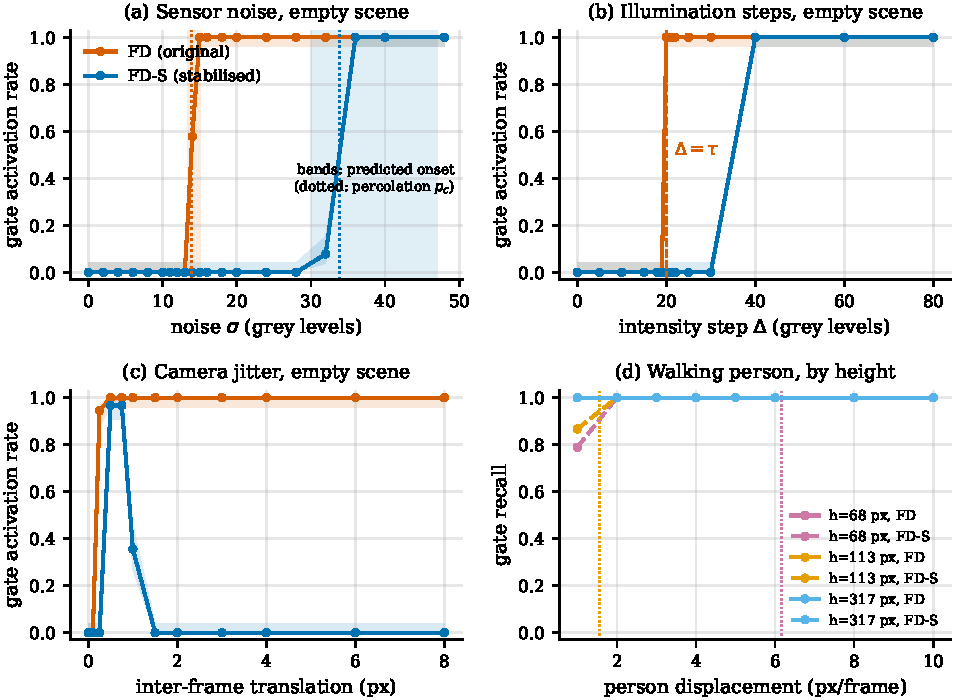
\includegraphics[width=\linewidth]{fig_envelope}
\caption{Operating envelope of \FD{} and \FDS{} (3 realisations $\times$ 30 transitions per point; shaded: 95\% Wilson intervals). (a)~Noise; bands mark the predicted onset for per-pixel exceedance probabilities between 0.01 and 0.1, dotted lines the percolation prediction. (b)~Illumination steps; the dashed line marks $\Delta=\tau$. (c)~Camera translation between consecutive frames. (d)~Walking persons of three heights; dotted lines mark the area-model bound $v^*$ where it is positive.}
\label{fig:envelope}
\end{figure}

The sweeps in \cref{fig:envelope} test the predictions of \cref{sec:envelope}:
\begin{itemize}
\item \emph{Noise.} \FD{} switches from never to always active at $\sigma=\MeasSigmaFD$ (50\% crossing), where the percolation criterion predicts $\PredSigmaPcFD$. \FDS{} switches at $\sigma=\MeasSigmaFDS$, predicted $\PredSigmaPcFDS$. The rectification bias thus accounts quantitatively for the difference in noise tolerance.
\item \emph{Illumination.} \FD{} fires from $\Delta=\MeasIllumFD$ on, which matches the prediction $\Delta>\tau=20$ up to the integer rounding of the OpenCV pipeline. \FDS{} tolerates steps of up to 30 grey levels and fires beyond (crossing at \MeasIllumFDS). For large steps, the neighbourhoods of saturated regions change by less than the offset, and after smoothing such partially clipped pixels escape the saturation mask. The illumination scenario of the benchmark (steps of $+32$ and $-50$) does not trigger \FDS, but its immunity is not complete.
\item \emph{Camera jitter.} \FD{} fires from translations of \MeasJitterFD\,px on, the same order of magnitude as the estimate $\delta^*\approx\PredJitter$\,px. \FDS{} suppresses translations of 1.5\,px and more completely but fires in a band around 0.5--1\,px. Such shifts already exceed the threshold at strong edges, yet they are too small for a reliable half-resolution estimate, so the compensation is rejected or inaccurate. This band explains the residual false-positive rate of \GateFprJitterFDS{} in the jitter scenario.
\item \emph{Size and speed.} All three persons trigger \FD{} already at 1\,px/frame, far below the area-model bounds of \PredSpeedA{} and \PredSpeedB\,px/frame for heights of \HeightA{} and \HeightB\,px. The textured interior of the silhouette changes many more pixels than the two edge strips, so the bound is tight only for weakly textured objects. \FDS{} is slightly less sensitive to the smallest persons at 1\,px/frame, because its signed difference lacks the positive bias that helps \FD.
\end{itemize}

\noindent \Cref{fig:pipeline} illustrates the difference on a frame of the jitter-and-walk scenario: \FD{} marks edges all over the scene, whereas the change mask of \FDS{} is dominated by the walking person.

\begin{figure}[t]
\centering
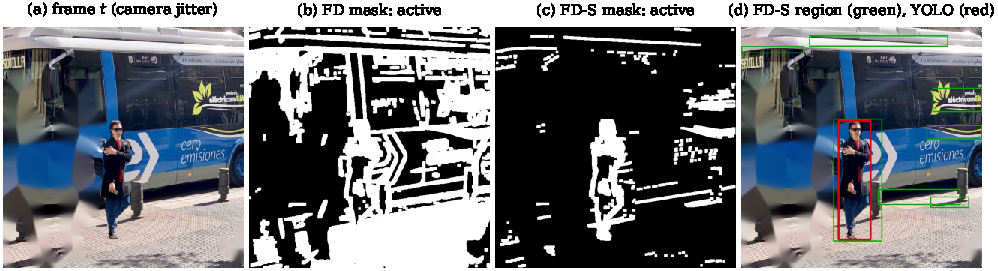
\includegraphics[width=\linewidth]{fig_pipeline}
\caption{A frame of the jitter-and-walk scenario (estimated camera shift \PipelineShift\,px). \FD{} marks edges all over the scene; \FDS{} compensates the shift and its mask is dominated by the walking person, with small residuals at the strongest edges. In (d) the red box is the YOLOv8m detection and the green boxes are the \FDS{} change regions.}
\label{fig:pipeline}
\end{figure}

\subsection{System level}\label{sec:res_system}
\begin{table}[t]
\centering
\caption{System-level results on the controlled benchmark ($K=\RefreshK$, $M=1$). Stale frames: frames without a person on which a box is reported. Latencies in frames relative to the every-frame detector. Time: measured gate costs plus measured detector costs of the invoked frames.}
\label{tab:policies}
\resizebox{\linewidth}{!}{\begin{tabular}{@{}lccccccccc@{}}
\toprule
Policy & $r$ & Recall & Stale & Mean & Max & Entry & Exit & Time & Speed- \\
 & & & frames & IoU & age & lat. & lat. & (s) & up \\
\midrule
Every frame & 1.000 & 0.998 & 0 & 0.981 & 0 & 0 & 0 & 628.3 & 1.00 \\
Fixed rate, $N=2$ & 0.500 & 0.997 & 0 & 0.938 & 1 & 0 & 0 & 313.3 & 2.01 \\
Gated, FD (original) & 0.629 & 0.997 & 0 & 0.981 & 14 & 1 & 0 & 395.0 & 1.59 \\
Gated, FD-S (stabilised) & 0.542 & 0.997 & 0 & 0.981 & 14 & 1 & 0 & 342.6 & 1.83 \\
Gated, MOG2 & 0.557 & 0.997 & 5 & 0.973 & 14 & 1 & 6 & 356.8 & 1.76 \\
\bottomrule
\end{tabular}
}
\end{table}

\Cref{tab:policies} compares the policies at the default setting. With \FDS{} the detector runs on \PolRatioFDS{} of the frames (\PolCallsFDS{} calls), and the system still matches the every-frame output: recall \PolRecallFDS{} vs.\ \PolRecallEvery, the same mean IoU (\PolIouFDS), no stale frames and no exit latency. The maximum age is $K-1=14$ frames, as guaranteed by Proposition~\ref{prop:guarantees}. The one-frame entry latency arises because the first visible sliver of an entering person changes fewer than $A_{\min}$ pixels. \FD{} reaches the same accuracy but needs \PolCallsFD{} calls because of its jitter triggers (speed-up \PolSpeedFD{} instead of \PolSpeedFDS). MOG2 did not register the person leaving the image, so its last box remained for \PolExitMOG{} frames until the refresh.

\Cref{fig:scenarios} and \cref{tab:scenario_results} break the invocation ratio down by scenario. Static scenarios cost $\lceil T/K\rceil/T=0.067$ with every gate, the lower bound of Proposition~\ref{prop:guarantees}, except for \FD{} under camera jitter and MOG2 under illumination steps. Scenarios with continuous motion reach the upper bound $1/M=1$.

\begin{figure}[t]
\centering
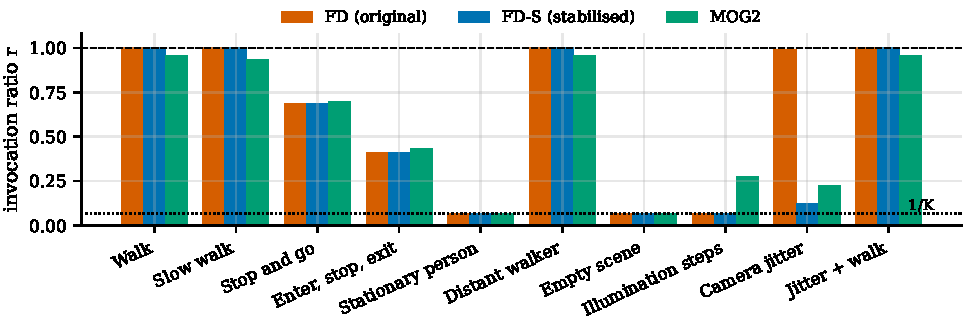
\includegraphics[width=\linewidth]{fig_scenarios}
\caption{Invocation ratio per scenario ($K=\RefreshK$, $M=1$). The dotted line marks the lower bound $1/K$, the dashed line the upper bound $1/M$.}
\label{fig:scenarios}
\end{figure}

\begin{table}[t]
\centering\small
\caption{Invocation ratio and frame recall per scenario ($K=\RefreshK$, $M=1$); recall is undefined without a person.}
\label{tab:scenario_results}
\begin{tabular}{@{}lcccccc@{}}
\toprule
 & \multicolumn{3}{c}{Invocation ratio $r$ ($K=15$)} & \multicolumn{3}{c}{Frame recall} \\
\cmidrule(lr){2-4}\cmidrule(l){5-7}
Scenario & FD & FD-S & MOG2 & FD & FD-S & MOG2 \\
\midrule
Walk & 1.000 & 1.000 & 0.956 & 1.000 & 1.000 & 1.000 \\
Slow walk & 1.000 & 1.000 & 0.933 & 1.000 & 1.000 & 1.000 \\
Stop and go & 0.689 & 0.689 & 0.700 & 1.000 & 1.000 & 1.000 \\
Enter, stop, exit & 0.411 & 0.411 & 0.433 & 0.973 & 0.973 & 0.973 \\
Stationary person & 0.067 & 0.067 & 0.067 & 1.000 & 1.000 & 1.000 \\
Distant walker & 1.000 & 1.000 & 0.956 & 1.000 & 1.000 & 1.000 \\
Empty scene & 0.067 & 0.067 & 0.067 & -- & -- & -- \\
Illumination steps & 0.067 & 0.067 & 0.278 & -- & -- & -- \\
Camera jitter & 0.989 & 0.122 & 0.222 & -- & -- & -- \\
Jitter + walk & 1.000 & 1.000 & 0.956 & 1.000 & 1.000 & 1.000 \\
\bottomrule
\end{tabular}

\end{table}

\Cref{fig:tradeoff}(a,b) compares the policy families across budgets. At IoU $\ge0.5$, fixed-rate subsampling is as good as gating with $M=1$ (\FixedRecallAtFDS{} at the budget of \FDS), but it degrades localisation (mean IoU \FixedIouAtFDS{} vs.\ \PolIouFDS). With larger $M$ the gated policies dominate: at $M=2$ \FDS{} keeps a recall of \PolRecallFDSMTwo{} at $r=\PolRatioFDSMTwo$ (fixed rate: \FixedRecallAtFDSMTwo), and at $M=4$ it keeps \PolRecallFDSMFour{} at $r=\PolRatioFDSMFour$ (fixed rate: \FixedRecallAtFDSMFour).

\begin{figure}[t]
\centering
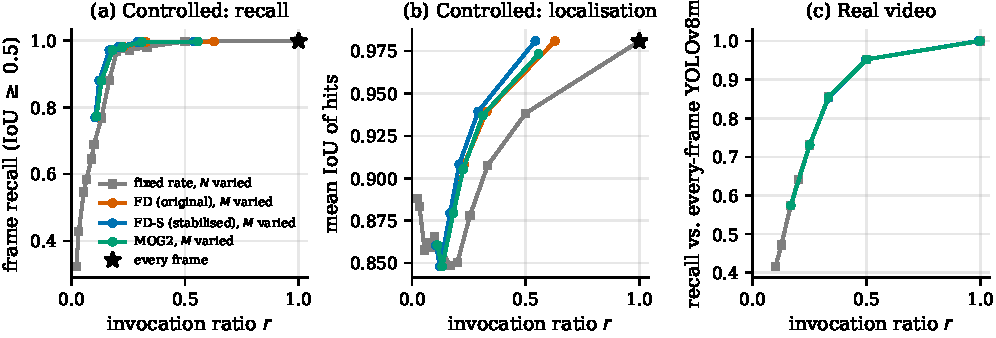
\includegraphics[width=\linewidth]{fig_tradeoff}
\caption{Accuracy versus detector budget. (a,b)~Controlled benchmark: gated policies with $K=\RefreshK$ and $M\in\{1,2,3,4,6,8\}$ against fixed-rate subsampling; (b)~shows the mean IoU of matched frames, i.e.\ localisation quality. (c)~Real video with $K=10$ and $M\in\{1,\dots,6\}$: the scene is almost always in motion, and all gated policies coincide with fixed-rate subsampling.}
\label{fig:tradeoff}
\end{figure}

\subsection{Cost model and online behaviour}\label{sec:res_cost}
On \EtoeFrames{} frames of the benchmark, the online system with \FD{} made \EtoeCallsFD{} detector calls and took \EtoeMeasuredFD\,s, against \EtoeEstimatedFD\,s estimated by the cost model (\EtoeErrFD\%). With \FDS{} it made \EtoeCallsFDS{} calls in \EtoeMeasuredFDS\,s against \EtoeEstimatedFDS\,s (\EtoeErrFDS\%). The decisions were identical to the offline replay (\EtoeMismatchFD{} and \EtoeMismatchFDS{} mismatches). The estimate is slightly pessimistic because the per-call costs were recorded while the machine was more heavily loaded (mean \YoloMs\,ms per call).

\subsection{Real video}\label{sec:res_video}
On \code{vtest.avi} every frame contains persons (\VtPersons{} on average), and the gates are active on \VtActiveFD{} (\FD), \VtActiveFDS{} (\FDS) and \VtActiveMOG{} (MOG2) of the frames (\cref{tab:video}). With $M=1$ the invocation ratio is therefore close to one and gating saves nothing; the gate's own cost even makes it marginally slower (speed-up \VtSpeedFDS{} with \FDS). With $M=2$ and $M=3$ the gated policies coincide with fixed-rate subsampling (recall \VtRecallFDSTwo{} at $r=\VtRatioFDSTwo$ and \VtRecallFDSThree{} at $r=\VtRatioFDSThree$), exactly as Proposition~\ref{prop:guarantees} predicts for continuous motion. Agreement at a given budget is lower than on the controlled benchmark: at \VtFps\,FPS a skipped frame is already 100\,ms old, and the detector flickers on small, partly occluded pedestrians.

\begin{table}[t]
\centering\small
\caption{Real video (\code{vtest.avi}, \VtFrames{} frames): agreement with YOLOv8m run on every frame ($K=10$).}
\label{tab:video}
\begin{tabular}{@{}lccccc@{}}
\toprule
Policy & $r$ & Recall & Precision & F1 & Speed-up \\
\midrule
Every frame & 1.000 & 1.000 & 1.000 & 1.000 & 1.00 \\
Fixed rate, $N=2$ & 0.501 & 0.952 & 0.954 & 0.953 & 2.00 \\
Fixed rate, $N=3$ & 0.333 & 0.855 & 0.854 & 0.854 & 3.00 \\
Fixed rate, $N=4$ & 0.250 & 0.731 & 0.734 & 0.732 & 4.00 \\
Gated, FD (original), $M=1$ & 0.997 & 1.000 & 1.000 & 1.000 & 1.00 \\
Gated, FD (original), $M=2$ & 0.501 & 0.952 & 0.954 & 0.953 & 1.99 \\
Gated, FD (original), $M=3$ & 0.333 & 0.855 & 0.854 & 0.854 & 2.98 \\
Gated, FD-S (stabilised), $M=1$ & 0.994 & 1.000 & 1.000 & 1.000 & 0.99 \\
Gated, FD-S (stabilised), $M=2$ & 0.498 & 0.952 & 0.954 & 0.953 & 1.95 \\
Gated, FD-S (stabilised), $M=3$ & 0.333 & 0.853 & 0.853 & 0.853 & 2.88 \\
Gated, MOG2, $M=1$ & 0.999 & 1.000 & 1.000 & 1.000 & 0.98 \\
Gated, MOG2, $M=2$ & 0.501 & 0.952 & 0.954 & 0.953 & 1.91 \\
Gated, MOG2, $M=3$ & 0.333 & 0.855 & 0.854 & 0.854 & 2.82 \\
\bottomrule
\end{tabular}

\end{table}


\clearpage

\section{Discussion}\label{sec:discussion}

\paragraph{When does gating pay off?} The invocation ratio is a property of the scene as much as of the system: by Proposition~\ref{prop:guarantees} it lies between $1/K$ when nothing moves and $1/M$ under continuous motion. On the controlled benchmark the \FDS-gated system sends \PolRatioFDS{} of the frames to the detector and reproduces the every-frame output almost exactly (recall \PolRecallFDS{} vs.\ \PolRecallEvery, mean IoU \PolIouFDS{} vs.\ \PolIouEvery). Fixed-rate subsampling with the same budget reaches the same recall at IoU $\ge0.5$ (\FixedRecallAtFDS), because a box that is one frame old still overlaps a walking person sufficiently. Its boxes, however, lag behind moving persons: the mean IoU drops to \FixedIouAtFDS{} at the same budget and to \PolIouFixedThree{} for every third frame. The gated policy concentrates staleness where it is harmless, in periods without motion. Recall at a lenient IoU threshold alone would hide this difference, yet applications that crop persons, count line crossings or estimate positions depend on localisation. At smaller budgets the minimum interval $M$ turns the gate into a clear improvement: with $M=4$, \FDS{} keeps a recall of \PolRecallFDSMFour{} at $r=\PolRatioFDSMFour$, where fixed-rate subsampling with the same budget reaches \FixedRecallAtFDSMFour{} (\cref{fig:tradeoff}a), because the gate spends the budget on the frames that change.

\paragraph{Robustness is a cost issue.} Every false trigger costs a full detector call. Under camera jitter \FD{} triggers on almost every frame, so the gated system becomes as expensive as running the detector on every frame (\cref{tab:scenario_results}). \FDS{} reduces the invocation ratio of that scenario by an order of magnitude while keeping recall on the walker filmed by the same jittering camera. Over the benchmark, \FDS{} needs \PolCallsFDS{} detector calls instead of \PolCallsFD{} at identical recall and localisation, and in the end-to-end run the measured time drops from \EtoeMeasuredFD\,s to \EtoeMeasuredFDS\,s. MOG2 is not a better gate for this purpose: it is the most expensive, it absorbs illumination steps only gradually, it misses part of the slow motion, and it kept a box for \PolExitMOG{} frames after the person had left.

\paragraph{Busy scenes.} Gating cannot save anything when something moves in almost every frame: on \code{vtest.avi} the gate is active on \VtActiveFDS{} of the frames. The minimum interval then acts as a cost cap, and the policy degrades gracefully into fixed-rate subsampling at rate $1/M$ instead of into running the detector on every frame. For such scenes the next step is to make each detector call cheaper, for example by running the detector on the motion regions only, or to extrapolate boxes between calls with a tracker.

\paragraph{Deployment guidance.} The analysis translates into a short checklist:
\begin{enumerate}
\item Measure $C_y$ and $C_m$ on the target hardware. Gating pays off whenever $r<1-C_m/C_y$ (\cref{eq:cost}), which holds by a wide margin for CPU inference; on a GPU $C_y$ shrinks and the margin narrows.
\item Derive $K$ from the oldest box the application accepts: $K=\lfloor s_{\max}f\rfloor+1$, e.g.\ $K=16$ for 0.5\,s at 30\,FPS.
\item Derive $M$ from the compute budget: under continuous motion the detector runs on every $M$-th frame.
\item Use \FDS{} whenever the camera can vibrate (poles, vehicles, slamming doors) or the lighting can change (clouds, switched lights); plain \FD{} suffices only for rigid indoor mounts with stable lighting.
\item Check $A_{\min}$ against the smallest person that must be detected with the area model~\eqref{eq:area}; lowering $A_{\min}$ recovers small or slow persons at the price of more noise triggers.
\item Keep the per-frame record (reason, age); downstream logic can then treat retained boxes differently from fresh ones.
\end{enumerate}

\paragraph{Limitations and threats to validity.}
\begin{itemize}
\item The controlled benchmark uses one background and one rigid, alpha-composited person without articulation, shadows or motion blur; noise is Gaussian and independent; jitter is a pure translation. Its results explain mechanisms rather than predict field performance. A walking person with moving limbs changes more pixels than the rigid cut-out, so the size and speed limits are conservative.
\item \FDS{} was designed with the failure modes of this benchmark in view, which risks overfitting. The real video was held out, but it has no annotations and contains no notable jitter or illumination events.
\item The reference in the real video is the detector itself, so the numbers measure agreement, not accuracy; detector flicker between consecutive frames lowers the agreement of every subsampling policy.
\item Timings come from one CPU thread of a shared machine; ratios such as $r$ and $C_m/C_y$ transfer better than absolute times.
\item \FDS{} still triggers for inter-frame translations of about 0.5--1\,px (\cref{fig:envelope}c), where half-resolution phase correlation is not accurate enough; full-resolution or iterative refinement~\cite{lucas1981iterative,evangelidis2008ecc} would address this at a higher cost. Rotation, zoom and parallax are not modelled.
\item The percolation estimate of the noise onset neglects the spatial correlation introduced by smoothing.
\end{itemize}

\paragraph{Future work.} A tracker such as SORT~\cite{bewley2016sort} could extrapolate boxes between detector calls instead of retaining them. The noise level could be estimated online to adapt $\tau$ through~\eqref{eq:bias}. The policies should also be evaluated on annotated real footage and measured on embedded hardware.


\newpage

\section{Conclusion}\label{sec:conclusion}
A motion gate in front of a person detector is simple to build, but whether it is safe and worthwhile depends on quantities that the original prototype did not control. With a refresh interval $K$ and a minimum interval $M$, the age of every reported box is bounded by $K-1$ frames and the detector load by $1/M$, and the load falls to $1/K$ when the scene is static. The weaknesses of frame differencing are predictable: a rectification bias sets its noise limit, any illumination step above the threshold triggers it, and sub-pixel camera motion triggers it. A stabilised gate that smooths signed differences, registers frames under an edge-based model selection, removes intensity offsets and propagates the registration error into the threshold removes most of these false triggers for a few milliseconds per frame. On the controlled benchmark the stabilised gate reproduces the every-frame output while calling the detector on \PolRatioFDS{} of the frames; at smaller budgets, the rate-limited gate is clearly better than fixed-rate subsampling. The accompanying package, tests and benchmark make every number of this paper reproducible with one command.


% ------------------------------------------------------------
% Bibliography
% ------------------------------------------------------------
\clearpage
\printbibliography[heading=bibintoc,title={References}]

% ------------------------------------------------------------
% Appendix
% ------------------------------------------------------------
\clearpage
\appendix

\section{Reproducibility}\label{app:repro}
\begin{lstlisting}[language=bash]
pip install -e ".[benchmark,dev]"   # package, benchmark and test dependencies
pytest                               # 28 unit tests
python -m benchmark.run              # all results, tables and figures
cd paper && latexmk -pdf main.tex    # this document
\end{lstlisting}
The benchmark expects \code{weights/yolov8m.pt}, \code{weights/yolov8n-seg.pt} and \code{data/vtest.avi} (download instructions in the README). Realisation $i$ uses seed $20260922+i$, and every scenario draws from its own random stream, so results do not depend on the order of execution. Detector outputs are cached in \code{results/cache}; raw results are stored as CSV and JSON in \code{results/}, and \code{results/metadata.json} records software versions and parameters. The complete run took about 35 minutes on one CPU thread. All numbers in this paper are read from \code{paper/generated/} and were not edited by hand.

\section{Review of the original prototype}\label{app:review}
Re-running the original script reproduced its counts exactly (84 of 144 frames sent to the detector) and a speed-up of 1.70 instead of the reported 1.71. The main changes and their reasons:
\begin{itemize}
\item \emph{Evaluation design.} Both systems were perfect on six short scenarios, so the benchmark could not discriminate between policies. It was replaced by ten longer scenarios with harder cases, a fixed-rate baseline at equal budget, operating-envelope sweeps and a real video.
\item \emph{Statistics.} The five seeds varied only the sensor noise; the new realisations also vary the camera jitter, and all rates carry confidence intervals. Recall was reported as 0.0 for scenarios without a person, where it is undefined; such entries are now marked as undefined.
\item \emph{Flat ablation.} Identical results for thresholds between 5 and 30 reflected trivially separable scenarios rather than robustness; the sweeps now locate the actual breakdown points and compare them with theory.
\item \emph{Camera jitter.} The failure was reported but not explained; it is now explained analytically (\cref{sec:envelope}) and addressed by \FDS.
\item \emph{Scheduler.} A rate limit $M$ was added and the guarantees are proven.
\item \emph{Software.} The script became a tested package with a command-line tool; the original detector is kept in \code{legacy/} for reference. A mis-attributed citation of the background-subtraction survey was corrected, and hard-coded numbers and dates were replaced by generated values.
\end{itemize}


% ------------------------------------------------------------
% Lists
% ------------------------------------------------------------
\clearpage
\phantomsection
\addcontentsline{toc}{section}{List of Figures}
\listoffigures

\clearpage
\phantomsection
\addcontentsline{toc}{section}{List of Tables}
\listoftables


\end{document}
